\section{Related Work}

The field of Legal Judgment Prediction (LJP) through AI has progressed significantly over the last few years. Traditionally the domain of legal experts, LJP systems offer potential benefits for practitioners and the public, particularly in managing overwhelming caseloads in various jurisdictions.
%
Foundational studies by \cite{aletras2016predicting}, \cite{chalkidis2019neural}, and \cite{feng2021recommending} established the methodologies for LJP and highlighted the critical need for explainability in AI-generated predictions. Benchmark datasets such as CAIL2018 \cite{xiao2018cail2018, zhong-etal-2020-nlp}, ECHR-CASES \cite{chalkidis2019neural, aletras2016predicting, medvedeva2020using}, and others have propelled research by providing a foundation for model evaluation. Despite these advances, challenges persist in achieving machine performance comparable to human expertise.

% %%%%%%%%%%%%%%%%%%%%%%%%%%%%%%%%%%%%
% \begin{figure}[t] % [h] specifies the placement of the figure
%     \centering % Centers the figure
%     % \begin{tcolorbox}[colframe=black, colback=white, boxrule=1pt, arc=0mm, outer arc=0mm]
%     % \fbox{ 
%     \includegraphics[width=\linewidth]{figures/NyayaAnumana_flow.pdf} % Adjust width as needed
%     % }
%     % \end{tcolorbox}
%     % 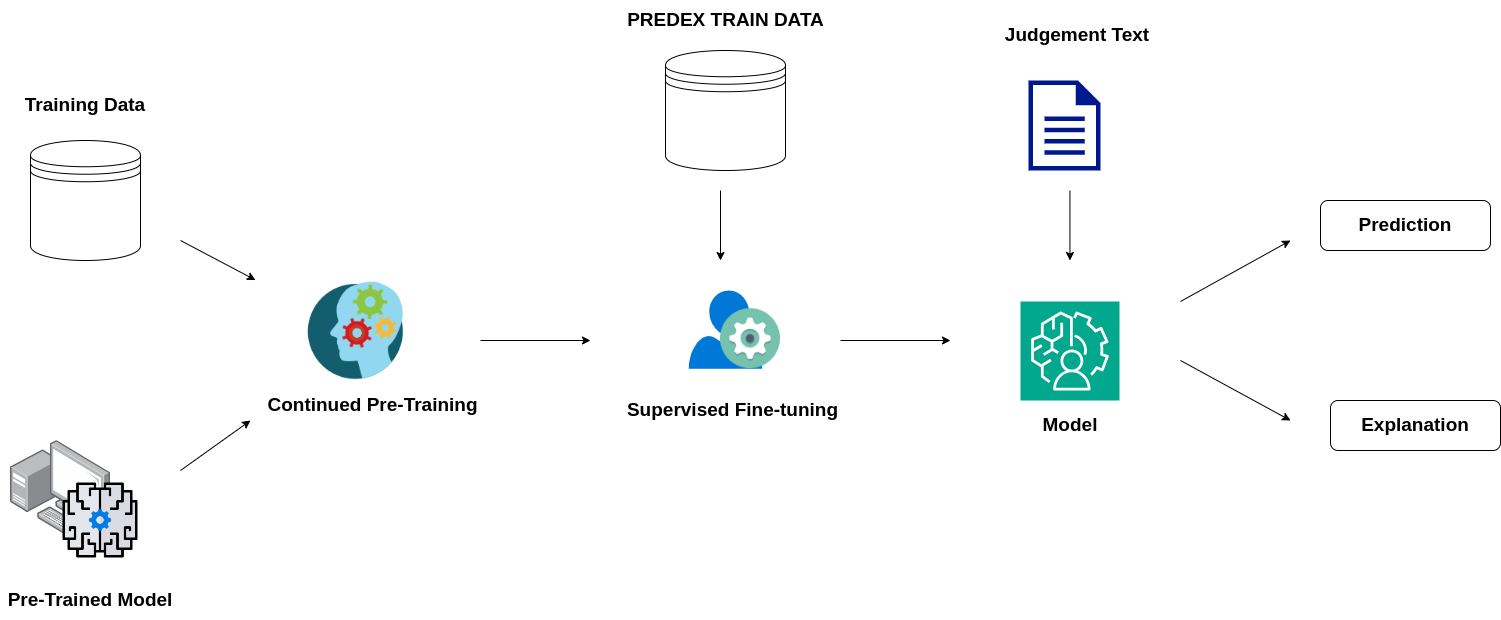
\includegraphics[width=0.5\textwidth]{figures/LLMs_part.drawio.png} 
%     \caption{Illustration of the LJP Task Framework.}
%     \label{fig:task-framework} % For referencing the figure
% \end{figure}
% %%%%%%%%%%%%%%%%%%%%%%%%%%%%%%%%%%%%


% %%%%%%%%%%%%%%%%%%%%%%%%%%%%%%%%%%%%
% \begin{figure*}[t] % [h] specifies the placement of the figure
%     \centering % Centers the figure
%     \includegraphics[width=\linewidth]{figures/NyayaAnumana_Flow.drawio_new.pdf} % Adjust width as needed
  
%     \caption{Illustration of the LJP Task Framework.}
%     \label{fig:task-framework} % For referencing the figure
% \end{figure*}
% %%%%%%%%%%%%%%%%%%%%%%%%%%%%%%%%%%%%

In the Indian context, significant contributions include PredEx \cite{nigam2024legaljudgmentreimaginedpredex} and ILDC \cite{malik-etal-2021-ildc}, which emphasize the importance of explainability in AI systems for legal reasoning. Fact-based judgment prediction has gained prominence as a realistic approach to LJP, focusing on predictions derived from case facts rather than full case judgments. \citet{nigam-etal-2024-rethinking} and \citet{10.1145/3632754.3632765} explore LJP based on facts, arguing that this approach better simulates real-world scenarios. \citet{nigam2022nigam, nigam-etal-2023-nonet, nigam2023legal, malik2021semantic, ganguly2023legal, ghosh2023report} underscore the growing role of AI in Indian legal applications, demonstrating the utility of advanced models like LLMs in addressing the unique challenges of this domain. Furthermore, \citet{tiwari2024aalap} and \citet{huang2023lawyer} illustrate the potential of AI assistants in legal and paralegal functions, showcasing the applicability of AI in streamlining legal processes and improving access to justice.
%
Cross-jurisdictional research, such as \cite{zhao-etal-2018-learning}, demonstrates the adaptability of LJP models across different legal systems and languages. The multilingual aspects of LJP are addressed by studies such as \cite{kapoor-etal-2022-hldc}, which introduces a corpus for Hindi legal documents, and \cite{niklaus2021swiss}, which examines the Swiss legal system.
